\subsection{Previous Research on Gender Differences in Knowledge}
% Now I want to show you why this matters
% This application challenges a common finding in political science and public opinion research, namely that women know significantly less about politics than men. Some studies attribute this difference to a relative lack in resources like education, or a more general disdain for politics among women. However, others argued that the gender gap might be an artifact due to differential propensities to guess or the fact that knowledge questions do not address gender relevant knowledge. I examine the gender gap by proposing a new measure of political sophistication that focuses on how individuals describe their political attitudes and beliefs in their own words.
% Example for gender gap: Verba, Burns, Schlozman (1997), Mondak


\begin{frame}\centering\vfill
    \begin{center}
        \begin{tikzpicture}
            \node[anchor=south west,inner sep=0] (image) at (0,0) {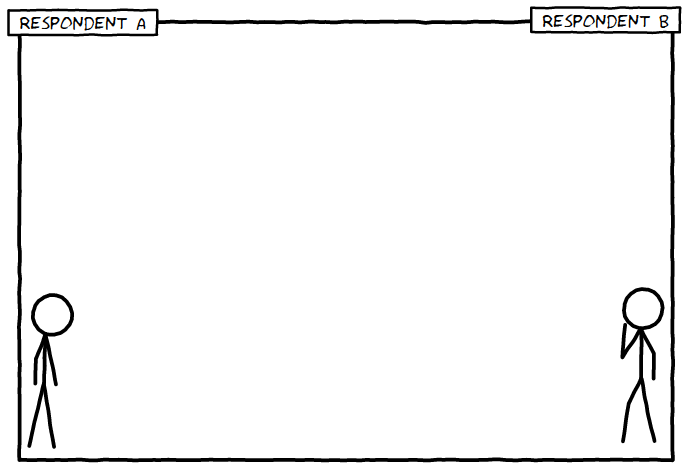
\includegraphics[width=\textwidth]{fig/Respondents_empty.png}};
            \node<2->[anchor=south west,inner sep=0] (vote) at (3.6,1.5) {
\includegraphics[width=.4\textwidth]{fig/Mind_the_gap1.jpg}};
            \node<3->[align=center,draw opacity=0,fill opacity=0.8,text opacity=1, white, fill=beamer@sbred] at (image.center) {\large Application
            \\\Large Assessing the Gender Gap
            \\\Large in Political Sophistication
            \\\vspace{1em}\\ (2012 ANES + 2015 YouGov)};
        \end{tikzpicture}
    \end{center}
\end{frame}
% Mention that results replicate in the remaining datasets


\begin{frame}{Previous Research on Gender Differences in Knowledge}
\visible<1->{\emph{General finding}: Women score \emph{lower} than men on \emph{conventional} measures of\\ \emph{political knowledge}
%\begin{itemize}\footnotesize
%\item \cite{converse1964nature}, \cite{verba1997knowing}
%% Converse: found gap, Verba: cannot be reduced, general distaste, Dow: women benefit differently from factors that increase knowledge
%\end{itemize}
}
\vspace{1em}
\visible<2->{\begin{center}
\emph{\faArrowRight}\hspace{1em} ``One of the \emph{most robust} findings in the study of political behavior.'' {\footnotesize\cite{dow2009gender}}
\end{center}}
\vspace{2em}
\visible<3->{\emph{Explanation 1:} Personality characteristics
%\begin{itemize}\footnotesize
%\item \cite{mondak2004knowledge}, \cite{mcglone2006stereotype}
%%Mondak: propensity to guess; McGlone: stereotype threat; Lizotte: propensity to guess due to risk aversion
%\end{itemize}
}\\\vspace{1em}
\visible<4->{\emph{Explanation 2:} Question content / gender-relevant knowledge
%\begin{itemize}\footnotesize
%\item \cite{stolle2010women}, \cite{dolan2011women}, \cite{jerit2017revisiting}
%% Stolle: practical issues (benefits/services); Dolan: women's representation; Jerit: Closing gap through learning)
%\end{itemize}
}
\end{frame}


\subsection{2012 ANES}

\begin{frame} %[allowframebreaks]
\frametitle{Gender Differences in Sophistication -- 2012 ANES}
  \begin{figure}
  \only<1>{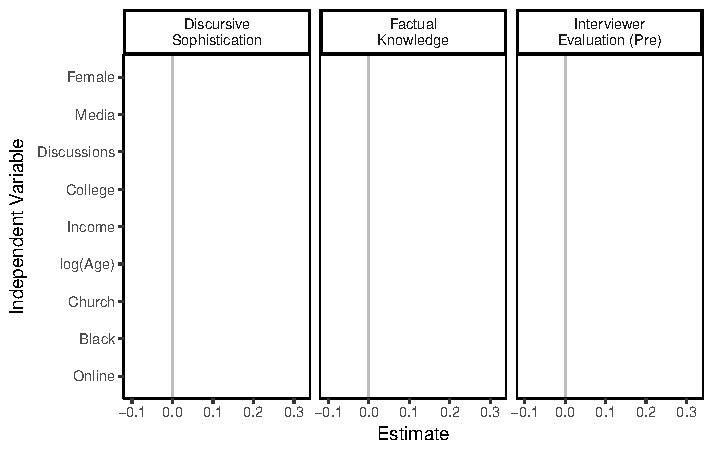
\includegraphics[width=.9\textwidth]{fig/determinants_0.pdf}}
  \only<2>{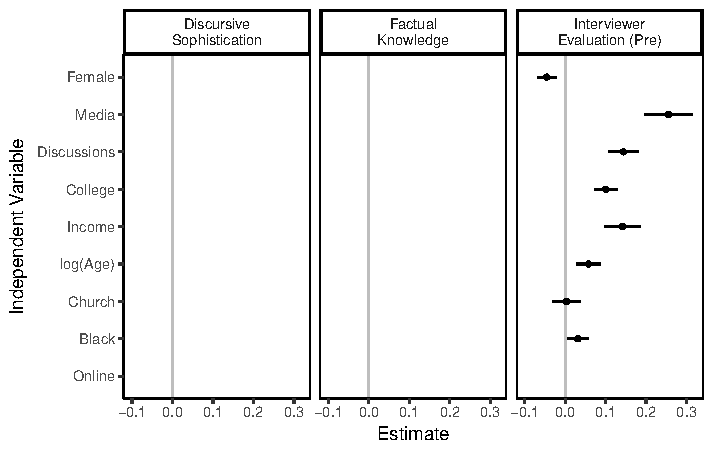
\includegraphics[width=.9\textwidth]{fig/determinants_1.pdf}}
  \only<3>{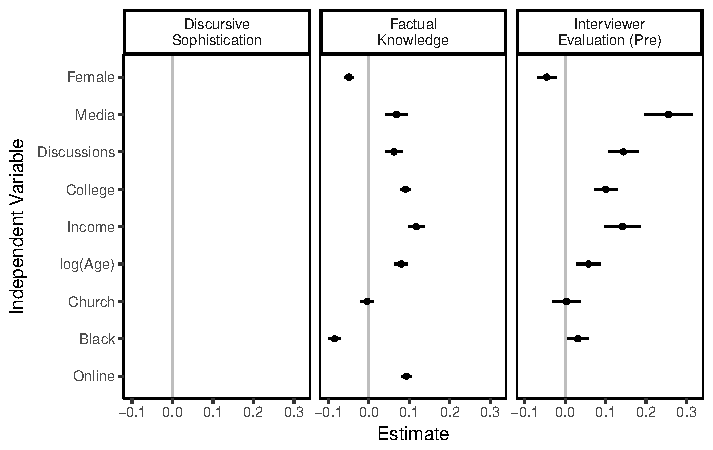
\includegraphics[width=.9\textwidth]{fig/determinants_2.pdf}}
  \only<4>{
\includegraphics[width=.9\textwidth]{fig/determinants_3.pdf}}
  \end{figure}
\end{frame}


\subsection{2015 YouGov}

\begin{frame} %[allowframebreaks]
\frametitle{Gender Differences in Sophistication -- 2015 YouGov}
  \begin{figure}
  \only<1>{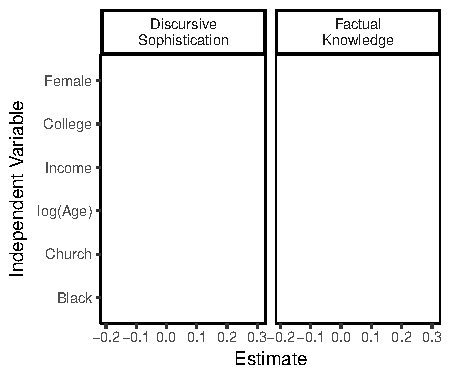
\includegraphics{fig/yg_determinants_empty.pdf}}
  \only<2>{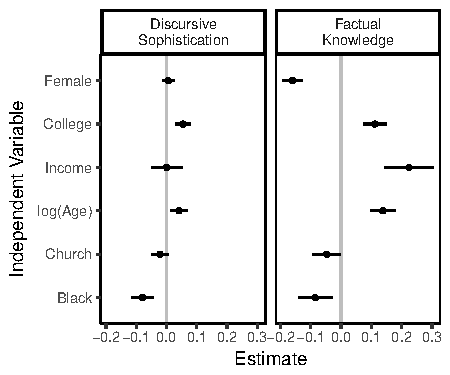
\includegraphics{fig/yg_determinants_pres.pdf}}
  \end{figure}
\end{frame}

%\begin{frame} %[allowframebreaks]
%\frametitle{Closing the Gender Gap}
%  \begin{figure}
%  
\includegraphics[width = \textwidth]{fig/closing_empty.pdf}
%  \end{figure}
%\end{frame}
%\begin{frame} %[allowframebreaks]
%\frametitle{Closing the Gender Gap}
%  \begin{figure}
%  
\includegraphics[width = \textwidth]{fig/closing.pdf}
%  \end{figure}
%\end{frame}

% TODO: add the yougov study as a replication

